\chapter{Uwaga (attention)}\label{rozdz:uwaga}

\section{Czemu konwolucja nie wystarcza?}

Konwolucja patrzy na stały, mały sąsiad (rozdział~\ref{rozdz:siec}). Tymczasem żeby ocenić, czy w danej klatce gra E3, sieć powinna
sprawdzić, czy gra też E2 (oktawę niżej, której alikwoty zlewają się z E3) i czy ta sama nuta trwała w poprzednich klatkach. To są
\emph{dalekie} zależności, a ich siła zależy od treści: oktawa jest ważna zawsze, ale tylko wtedy, gdy dwie nuty rzeczywiście grają razem.
Mechanizm, który wybiera, na co patrzeć, na podstawie treści, nazywamy \emph{uwagą}.

Po tym rozdziale umiesz: (i)~policzyć uwagę dla kilku elementów ręcznie, (ii)~uzasadnić, że wynik jest średnią ważoną wartości,
(iii)~wyjaśnić, skąd się bierze dzielenie przez $\sqrt{d}$, (iv)~policzyć liczbę parametrów warstwy uwagi i wskazać, jak nadać jej wiedzę o położeniu.

\section{Uwaga pojedynczego zapytania}

Każdy element sekwencji dostaje trzy wektory: \emph{zapytanie} $\vect q$ („czego szukam”), \emph{klucz} $\vect k$ („co oferuję”) i \emph{wartość} $\vect v$ („co przekazuję, gdy mnie wybierzesz”).
Powstają z wektora cech $\vect h$ przez trzy macierze: $\vect q=W_Q\vect h$, $\vect k=W_K\vect h$, $\vect v=W_V\vect h$ (rozdział~\ref{rozdz:wektory}).

\haslo{uwaga}
\begin{definicja}[Uwaga skalowana iloczynem skalarnym]\label{def:uwaga}
Dla zapytania $\vect q\in\R^d$, kluczy $\vect k_1,\dots,\vect k_n\in\R^d$ i wartości $\vect v_1,\dots,\vect v_n\in\R^{d_v}$ oraz opcjonalnych \emph{premii} $b_j\in\R$:
\begin{equation}
  s_j=\frac{\ip{\vect q}{\vect k_j}}{\sqrt d}+b_j,\qquad
  \alpha_j=\softmax(s)_j,\qquad
  \operatorname{Attn}(\vect q)=\sum_{j=1}^{n}\alpha_j\,\vect v_j .
\end{equation}
Liczby $\alpha_j$ nazywamy \emph{wagami uwagi}.
\end{definicja}

\begin{przyklad}[Trzy elementy, policzone ręcznie]\label{prz:uwaga}
Niech $d=2$, $\vect q=(1,0)$, klucze $\vect k_1=(1,0)$, $\vect k_2=(0,1)$, $\vect k_3=(1,1)$, wartości $\vect v_1=(1,0)$, $\vect v_2=(0,1)$, $\vect v_3=(2,2)$, premie $b=0$.
Wyniki $\ip{\vect q}{\vect k_j}=(1,0,1)$, dzielone przez $\sqrt2$: $s=(0{,}707;\,0;\,0{,}707)$. Wykładniki: $(2{,}028;\,1;\,2{,}028)$, suma $5{,}056$, wagi $\alpha=(0{,}401;\,0{,}198;\,0{,}401)$.
Wynik: $0{,}401\cdot(1,0)+0{,}198\cdot(0,1)+0{,}401\cdot(2,2)=(1{,}203;\;1{,}000)$.
Zapytanie $(1,0)$ „pasuje” do kluczy $1$ i $3$ (oba mają pierwszą współrzędną $1$), więc one dominują w wyniku. Gdyby klucz $3$ dostał premię $b_3=-1$, jego waga spadłaby do $0{,}198$ i wynik zmieniłby się na $(0{,}933;\,0{,}660)$.
\end{przyklad}

\begin{intuicja}
Uwaga to miękkie wyszukiwanie w słowniku: zapytanie porównujemy ze wszystkimi kluczami (iloczyn skalarny = podobieństwo), zamieniamy podobieństwa na wagi (softmax) i zwracamy średnią wartości ważoną tymi wagami.
Zamiast jednego wyniku „dokładnie to hasło” dostajemy mieszankę wszystkich, z naciskiem na najlepiej pasujące.
\end{intuicja}

\begin{twierdzenie}[Wynik uwagi to średnia ważona]\label{tw:uwaga-wypukla}
Wagi spełniają $\alpha_j>0$ i $\sum_j\alpha_j=1$, więc $\operatorname{Attn}(\vect q)$ leży w otoczce wypukłej wartości $\vect v_1,\dots,\vect v_n$: dla każdej współrzędnej $l$,
$\min_jv_{j,l}\le\operatorname{Attn}(\vect q)_l\le\max_jv_{j,l}$.
\end{twierdzenie}
\begin{pomyslDowodu}
Wagi są wynikiem softmaksa (tw.~\ref{tw:softmax}); średnia ważona dodatnimi wagami o sumie $1$ nie wychodzi poza zakres wartości.
\end{pomyslDowodu}
\begin{proof}
Z tw.~\ref{tw:softmax}(a): $\alpha_j>0$ i $\sum\alpha_j=1$. Niech $m=\min_jv_{j,l}$, $M=\max_jv_{j,l}$.
\begin{align*}
\operatorname{Attn}(\vect q)_l &= \sum_j\alpha_jv_{j,l}\le\sum_j\alpha_jM=M && \pow{($\alpha_j>0$, $v_{j,l}\le M$)}\\
\operatorname{Attn}(\vect q)_l &\ge \sum_j\alpha_jm=m. && \pow{(analogicznie)}
\end{align*}
Wynik leży więc między skrajnymi wartościami. Warstwa uwagi nie „wymyśla” nowych wartości spoza zakresu, tylko je miesza; to ona wybiera, w jakich proporcjach. To kończy dowód.
\end{proof}

\section{Dlaczego dzielimy przez $\sqrt{d}$}

\begin{twierdzenie}[Wariancja iloczynu skalarnego]\label{tw:wariancja}
Jeśli współrzędne $q_i,k_i$ są niezależnymi zmiennymi losowymi o średniej $0$ i wariancji $1$, to $\Exp[\ip{\vect q}{\vect k}]=0$ i $\Var(\ip{\vect q}{\vect k})=d$.
Zatem $\ip{\vect q}{\vect k}/\sqrt d$ ma wariancję $1$ niezależnie od $d$.
\end{twierdzenie}
\begin{pomyslDowodu}
Iloczyn skalarny to suma $d$ niezależnych składników $q_ik_i$, z których każdy ma średnią $0$ i wariancję $1$; wariancje niezależnych składników się dodają.
\end{pomyslDowodu}
\begin{proof}
Dla jednego składnika, z niezależności $q_i$ i $k_i$:
\begin{align*}
\Exp[q_ik_i] &= \Exp[q_i]\,\Exp[k_i]=0, && \pow{(niezależność)}\\
\Var(q_ik_i) &= \Exp[q_i^2k_i^2]=\Exp[q_i^2]\,\Exp[k_i^2]=1\cdot1=1. && \pow{(średnia $0$, więc $\Var=\Exp[\cdot^2]$)}
\end{align*}
Składniki są niezależne, więc wariancja sumy to suma wariancji: $\Var\big(\sum_iq_ik_i\big)=d$. Dzielenie przez $\sqrt d$ dzieli wariancję przez $d$ (stała wychodzi do kwadratu). To kończy dowód.
\end{proof}

W zwykłym języku: im dłuższe wektory, tym większe losowe wyniki iloczynów. Duże wyniki wpychają softmax w nasycenie (jedna waga bliska $1$, reszta $\approx0$), gdzie jego gradient zanika. Skalowanie utrzymuje wyniki w rozsądnym zakresie
(rys.~\ref{rys:uwaga}c: pomarańczowy rozrzut rośnie jak $\sqrt d$, niebieski, po skalowaniu, jest stały).

\section{Uwaga dla całej sekwencji i premie położenia}

Gdy każdy z $n$ elementów jest też zapytaniem, wszystko zapisujemy macierzowo: $Q,K,V\in\R^{n\times d}$ (wiersze to wektory), $\operatorname{Attn}(Q,K,V)=\softmax\!\big(QK^{\top}/\sqrt d+B\big)V$, gdzie softmax działa na każdy wiersz,
a $B\in\R^{n\times n}$ to macierz premii. Wynikiem jest nowy zestaw $n$ wektorów.

\begin{twierdzenie}[Bez premii uwaga nie zna kolejności]\label{tw:permutacje}
Niech $P$ będzie macierzą permutacji. Dla $B=0$: $\operatorname{Attn}(PQ,PK,PV)=P\,\operatorname{Attn}(Q,K,V)$.
\end{twierdzenie}
\begin{pomyslDowodu}
Permutacja wierszy $Q,K$ permutuje wiersze i kolumny macierzy wyników w ten sam sposób; softmax po wierszach tego nie zauważa.
\end{pomyslDowodu}
\begin{proof}
$(PQ)(PK)^\top=PQK^\top P^\top$, więc macierz wyników $S$ zamienia się w $PSP^\top$: wiersze i kolumny są przetasowane tak samo. Softmax liczony po wierszach przestawia kolumny wewnątrz wiersza bez zmiany wag, a $P$ przestawia wiersze:
$\softmax(PSP^\top)=P\,\softmax(S)\,P^\top$. Stąd
\begin{align*}
\operatorname{Attn}(PQ,PK,PV) &= P\,\softmax(S)\,P^\top P V && \pow{($P^\top P=I$)}\\
 &= P\,\operatorname{Attn}(Q,K,V). && \pow{(def.)}
\end{align*}
Przetasowanie wejścia tylko przetasowuje wyjście. To kończy dowód.
\end{proof}

W zwykłym języku: samo „co” nie mówi „gdzie”. Gdyby klatki wymieszać, uwaga nie zauważy. Dlatego dodajemy \emph{premię zależną od odległości} $b_{j-i}$ (wyuczoną liczbę dla każdej różnicy położeń): sieć może się nauczyć, że odległość $12$ półtonów (oktawa) jest szczególnie ważna,
albo że klatka sprzed $0{,}5$ s ma inną wagę niż sąsiednia. Niektóre pary można też zablokować, ustawiając $b=-\infty$ (waga wtedy dokładnie $0$): tak powstaje \emph{okno} $\abs{j-i}\le W$ (rys.~\ref{rys:uwaga}b), które w Gen~6 ma $W=43$ klatki ($\approx1$ s) i kosztuje $O(n(2W+1))$ zamiast $O(n^2)$.

\begin{figure*}[ht]
\centering
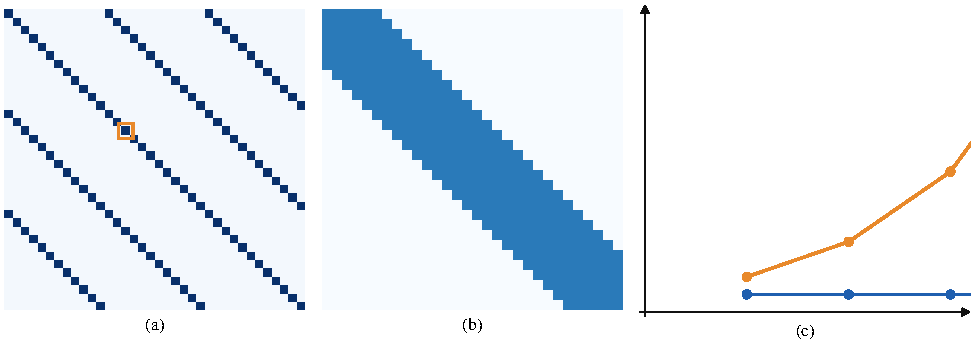
\includegraphics[width=\linewidth]{figures/uwaga.pdf}
\caption{(a) Zabawka: $36$ półtonów, a zapytanie i klucz to wskazanie klasy wysokości $(i\bmod12)$. Każdy wiersz macierzy wag $\alpha$ ma ciemne pola tylko dla tej samej klasy, czyli co $12$ półtonów: wysokość $14$ (pomarańczowa ramka)
patrzy na $2$, $14$ i $26$ --- uwaga potrafi „zobaczyć” oktawy. (b) Maska okna $\abs{t-u}\le5$ dla $30$ klatek: tylko pasmo wokół przekątnej ma niezerowe wagi. (c) Odchylenie standardowe $\ip{\vect q}{\vect k}$ dla wymiarów $d=4,16,64,256$ (oś pozioma $\log_2d$):
bez skalowania (pomarańczowa) rośnie jak $\sqrt d$, po podzieleniu przez $\sqrt d$ (niebieska) jest równe $1$. Obliczone z $10^5$ losowych par.}
\label{rys:uwaga}
\end{figure*}

\begin{figure}[ht]
\centering
\begin{tikzpicture}[>=Stealth,node distance=5mm,font=\small]
  \node[blok,minimum width=9mm] (h) {$H$};
  \node[blok,above right=2mm and 9mm of h,minimum width=9mm] (q) {$Q$};
  \node[blok,right=9mm of h,minimum width=9mm] (k) {$K$};
  \node[blok,below right=2mm and 9mm of h,minimum width=9mm] (v) {$V$};
  \node[blok,right=9mm of k,minimum width=16mm] (s) {$\softmax\!\big(\tfrac{QK^\top}{\sqrt d}+B\big)$};
  \node[blok,right=9mm of s,minimum width=9mm] (o) {$\times V$};
  \draw[wektor] (h)--(q); \draw[wektor] (h)--(k); \draw[wektor] (h)--(v);
  \draw[wektor] (q.east)--++(2mm,0)|-(s.west); \draw[wektor] (k)--(s);
  \draw[wektor] (s)--(o); \draw[wektor] (v.east)--++(2mm,0) -| ([xshift=3mm]o.south);
\end{tikzpicture}
\sidecaption{Przepływ danych jednej głowicy uwagi. Wektory cech $H\in\R^{n\times D}$ są rzutowane na $Q,K,V\in\R^{n\times d_h}$; iloczyny $QK^\top\in\R^{n\times n}$ (wyniki dopasowania), dzielone przez $\sqrt{d}$ i powiększone o premie $B$, przechodzą przez softmax
wiersz po wierszu; powstałe wagi mnożą $V$ i dają wyjście $n\times d_h$. \label{rys:uwaga-schemat}}
\end{figure}

\section{Wiele głowic i liczba parametrów}

Jedna uwaga potrafi śledzić jedną zależność naraz. \emph{Wielogłowicowa} uwaga dzieli wektor $D$-wymiarowy na $n_h$ części po $d_h=D/n_h$, w każdej liczy osobną uwagę (osobne $W_Q,W_K,W_V$ i osobne premie), skleja wyniki i mnoży przez $W_O$.
W Gen~6: $D=64$, $n_h=4$, $d_h=16$.

\begin{naliczbach}
Macierz $W_{QKV}\colon64\to192$ (trzy macierze naraz) ma $64\cdot192+192=12\,480$ parametrów; $W_O\colon64\to64$ ma $64\cdot64+64=4160$. Premie czasowe: $n_h(2W+1)=4\cdot87=348$; premie między wysokościami: $n_h(2S-1)=4\cdot105=420$
(dla $S=53$). Uwaga w czasie ma więc $12\,480+4160+348=16\,988$ parametrów, a uwaga między wysokościami $12\,480+4160+420=17\,060$ --- zgodnie z dodatkiem~\ref{dod:parametry}.
\end{naliczbach}

\begin{pulapka}
Wagi uwagi (rys.~\ref{rys:uwaga}a) bywają interpretowane jako „wyjaśnienie” decyzji modelu. To tylko część obrazu: po uwadze są jeszcze macierze $W_O$, normalizacja i kolejne warstwy, a każda głowica widzi inne części wektora. Wagi uwagi pokazują, skąd model brał informacje w jednym kroku, a nie dlaczego podjął decyzję.
\end{pulapka}

\section*{Podsumowanie}
\begin{itemize}
\item Uwaga: $\operatorname{Attn}(\vect q)=\sum_j\softmax(\ip{\vect q}{\vect k_j}/\sqrt d+b_j)\,\vect v_j$.
\item Wynik to średnia ważona wartości, więc nie wychodzi poza ich zakres (tw.~\ref{tw:uwaga-wypukla}).
\item Dzielenie przez $\sqrt d$ utrzymuje wariancję wyników na $1$ (tw.~\ref{tw:wariancja}).
\item Bez premii uwaga nie odróżnia kolejności (tw.~\ref{tw:permutacje}); premia zależna od odległości daje jej wiedzę o położeniu i pozwala wyróżnić oktawę lub zablokować dalekie pary (okno).
\item Wiele głowic = wiele zależności naraz; Gen~6: $n_h=4$, $d_h=16$.
\end{itemize}

\begin{sprawdz}
\begin{enumerate}
\item Dla $\vect q=(0,2)$, kluczy $(1,0),(0,1)$ i wartości $(5,0),(0,5)$ (z $d=2$) policz wagi i wynik uwagi.
\item Pokaż, że dodanie tej samej stałej $c$ do wszystkich premii $b_j$ nie zmienia wag $\alpha_j$.
\item Elementy mają $d=100$ i współrzędne $q_i,k_i$ o wariancji $1$. Jakie odchylenie standardowe ma $\ip{\vect q}{\vect k}$ bez skalowania, a jakie po skalowaniu?
\item Ile parametrów ma wielogłowicowa uwaga z $D=128$, $n_h=8$ (bez premii)?
\end{enumerate}
\end{sprawdz}

\subsection*{Rozwiązania}
\begin{enumerate}
\item $\ip{\vect q}{\vect k_j}=(0,2)$, dzielone przez $\sqrt2$: $(0;\,1{,}414)$, wykładniki $(1;\,4{,}113)$, suma $5{,}113$, wagi $(0{,}196;\,0{,}804)$. Wynik $0{,}196(5,0)+0{,}804(0,5)=(0{,}978;\,4{,}022)$.
\item Z tw.~\ref{tw:softmax}(b): $\softmax(s+c\vect1)=\softmax(s)$.
\item Bez skalowania $\sqrt{100}=10$; po skalowaniu $1$ (tw.~\ref{tw:wariancja}).
\item $W_{QKV}$: $128\cdot384+384=49\,536$; $W_O$: $128\cdot128+128=16\,512$; razem $66\,048$ (liczba głowic nie zmienia liczby parametrów, tylko sposób ich podziału).
\end{enumerate}
